\begin{center}
    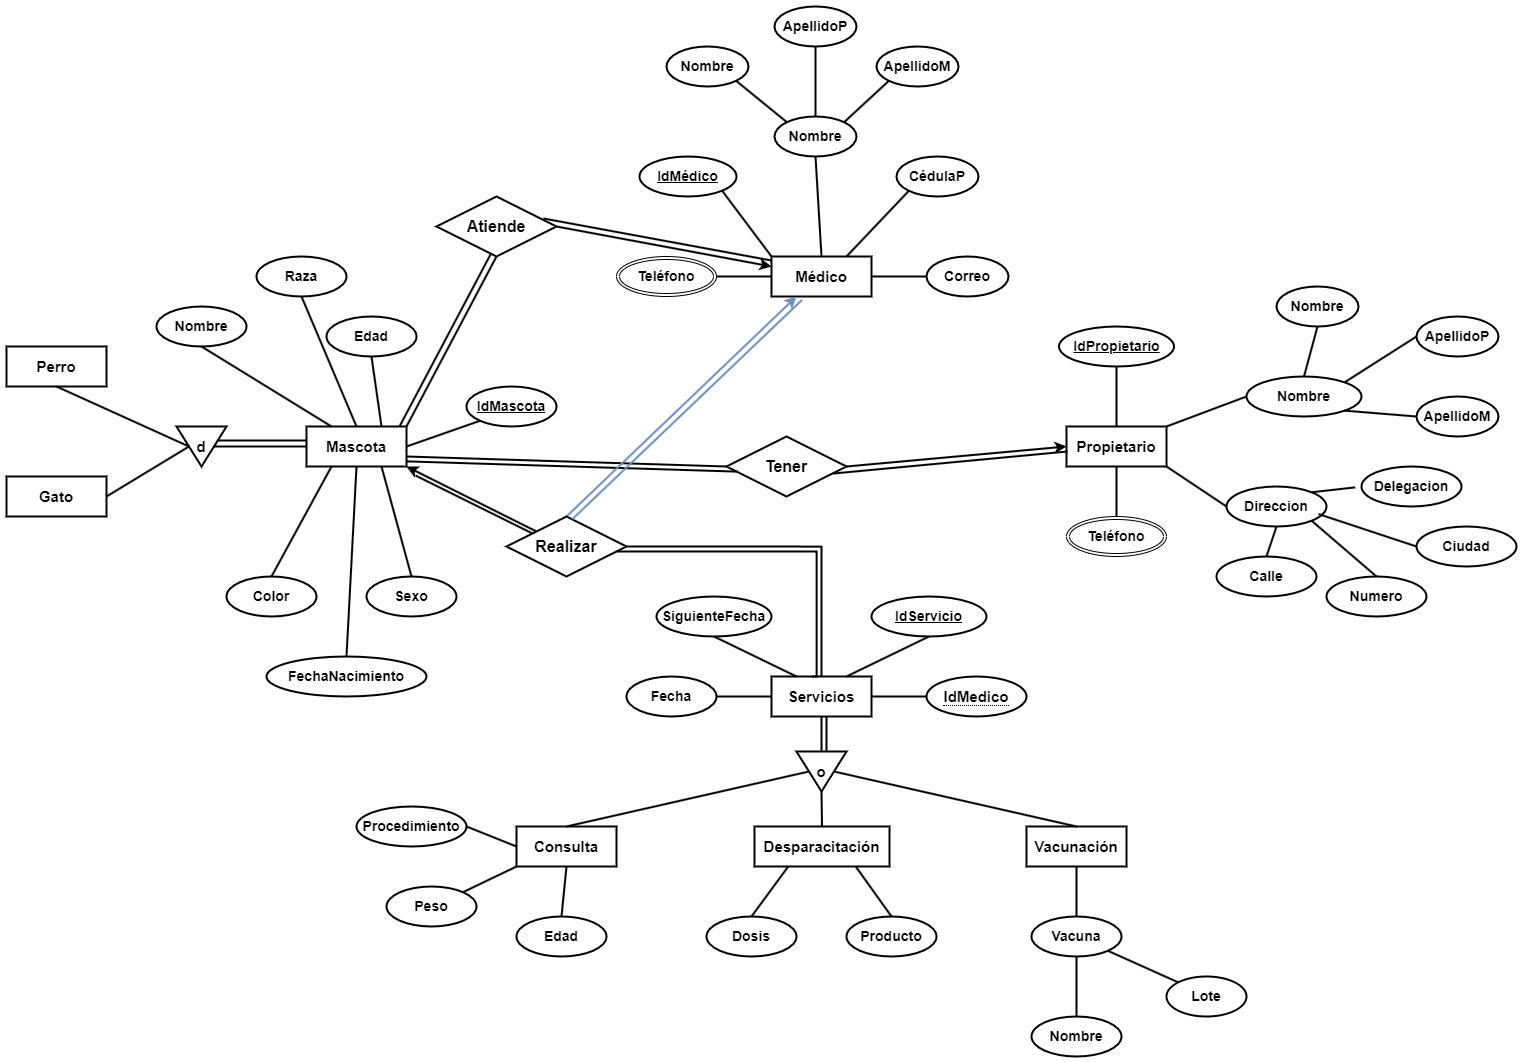
\includegraphics[width=10cm]{resources/Clinica-Veterinaria.png}
\end{center}

Propietario - Mascota: Un propietario puede tener muchas mascotas, y una mascota pertenece a un propietario (1:N). Ambos ocupan participación obligatoria

Mascota - Servicio: En este caso tenemos participación obligatoria de ambos lados y una mascota puede acudir a muchos servicios, el cuál, por la herencia puede ser uno o los tres servicios (por ejemplo, dos vacunas). 

Médico - Servicio: Indicado en azul, uno medico puede realizar muchos servicios obligatoriamente y el servicio(s) es realizado también obligatoriamente por el médico.

Médico- Mascota: Participación obligatoria de ambos lados. Un solo medico puede atender a muchas mascotas.

